\documentclass{article}

% if you need to pass options to natbib, use, e.g.:
\PassOptionsToPackage{numbers, compress}{natbib}
% before loading nips_2017
%
% to avoid loading the natbib package, add option nonatbib:
% \usepackage[nonatbib]{nips_2017}

\usepackage[final]{nips_2017}

% to compile a camera-ready version, add the [final] option, e.g.:
% \usepackage[final]{nips_2017}

\usepackage{amssymb,amsmath,amsfonts,graphicx,enumitem,amssymb, mathtools, bm,listings}
\usepackage[utf8]{inputenc} % allow utf-8 input
\usepackage[T1]{fontenc}    % use 8-bit T1 fonts
\usepackage{hyperref}       % hyperlinks
\usepackage{url}            % simple URL typesetting
\usepackage{booktabs}       % professional-quality tables
\usepackage{amsfonts}       % blackboard math symbols
\usepackage{nicefrac}       % compact symbols for 1/2, etc.
\usepackage{microtype}      % microtypography


\newcommand{\hba}{\textrm{HbA1c}}
\newcommand{\f}{f_{\mathrm{RBC}_{\mathrm{age}}}}
\newcommand{\dd}{\mathrm{d }}
\newcommand{\mean}{M_\mathrm{RBC}}
\newcommand\E{\mathbb{E}}
\newcommand\R{\mathbf{R}}
\newcommand\C{\mathbf{C}}
\newcommand\SM{\mathbf{S}}
\newcommand\T{^\top}
\newcommand{\st}{\text{subject to }}
\newcommand{\ip}[2]{\langle #1, #2 \rangle}
\newcommand{\twomat}[4]{\begin{bmatrix} #1 & #2 \\ #3 & #4 \end{bmatrix}}

\title{Inferring the age distribution of blood cells}

% The \author macro works with any number of authors. There are two
% commands used to separate the names and addresses of multiple
% authors: \And and \AND.
%
% Using \And between authors leaves it to LaTeX to determine where to
% break the lines. Using \AND forces a line break at that point. So,
% if LaTeX puts 3 of 4 authors names on the first line, and the last
% on the second line, try using \AND instead of \And before the third
% author name.

\author{
  Aodong Li\\  
  Computer Science Department\\
  New York University\\
  New York, NY 10003 \\
  \texttt{al5350@nyu.edu} \\
  %% examples of more authors
  %% \And
  %% Coauthor \\
  %% Affiliation \\
  %% Address \\
  %% \texttt{email} \\
  %% \AND
  %% Coauthor \\
  %% Affiliation \\
  %% Address \\
  %% \texttt{email} \\
  %% \And
  %% Coauthor \\
  %% Affiliation \\
  %% Address \\
  %% \texttt{email} \\
  %% \And
  %% Coauthor \\
  %% Affiliation \\
  %% Address \\
  %% \texttt{email} \\
}

\begin{document}
% \nipsfinalcopy is no longer used

\maketitle

\begin{abstract}
\hba\ is a measurement of the glycation percentage of hemoglobin  -- a specific kind of protein in blood cells. Glycation of proteins results from the chronic attachment of glucose in the bloodtream. It turns out that the measurement is highly correlated to the glucose concentration over the preceding 8--12 weeks and to the blood cell age distribution.
%is correlated to the glucose concentration over the preceeding 5-12 weeks, the measurement of \hba is predominantly used to moniter the long-term glycemic control for patients with diabetes. 
The relationship between \hba\ and the average glucose concentration has been rigorously investigated by \citet{nathan2008translating}. However, much detailed connection among \hba, varying glucose level, and the blood cell age distribution has not been touched yet. In this paper, we sought to define the mathematical relationship among these three factors and investigate the assumptions under which the inference of the blood cell age distribution is feasible. In particular, we define their connections as a convolution operation. Simulation results show that the proposed assumptions are consistent if the cell age distribution is uniform. Other theoretical aspects involving how to distinguish the uniform distribution and the finite exponential distribution, how to specify a linear programming problem for inferring a generic distribution, and the possibility of applying the pointwise deconvolution
%Fourier analysis
 are also investigated.
\end{abstract}

\section{Introduction}

Blood cells in the bloodstream are exposed to varying levels of sugar (glucose, $G(t)$). For healthy people, fingerstick capillary glucose concentration  has a mean of about $100$ mg/dL with a standard deviation of about $10$ mg/dL.  For people with type I diabetes, mean fingerstick glucose can be as high as $250$ mg/dL, and the standard deviation can be as high as $60$ mg/dL.

Due to the affinity of the molecular structures, glucose is automatically attached to some particular part of the proteins in blood cells. These proteins become glycated irreversibly at a rate that depends on $G(t)$. The glycation process is slow, and even the oldest cells rarely reach a $20\%$ level of glycation. The glycation process is never saturated.

We can take a blood sample and measure the overall glycated fraction of proteins in all the cells.  Blood cells contain various proteins. If the target protein is hemoglobin, its glycated form is called hemoglobin A1c, and the measurement is referred to as \hba.

Because the blood cells are in circulation for approximately $120$ days and the glycation is accumulated in the cells over this period, \hba\ has been standardized to monitor the long-term glycemic control according to \citet{berg2008haemoglobin}. Moreover, this accumulation process makes the concentration of \hba\ depend on both the glucose concentration $G(t)$ and the lifespan of blood cells. 

\citet{nathan2008translating}\cite{nathan2007relationship}\cite{nathan1984clinical} have studied rigorously the relationship between \hba\ and the average glucose concentration over the preceding 8--12 weeks, and confirmed the striking linear connection. To our knowledge, however, the precise interplay between \hba, $G(t)$, and the cell lifespan (or the age distribution $\f(t)$) has not been investigated in a much detailed manner.

In this paper, we sought to explore the precise mathematical relationship among \hba, $G(t)$, and $\f(t)$ whilst establishing the necessary assumptions to make the inference of $\f(t)$ possible. In summary, we make the following contributions:  
\begin{enumerate}
%\item The glycation rate $v(t)$ is specified to be linear with $G(t)$ as an assumption.
\item We define the mathematical relationship among these factors as a convolution operation. In particular, \hba\ is a convolution of $G(t)$ and $\f(t)$.
\item When $\f$ is uniform, we show that it can be inferred easily with one measurement \hba.
\item Based on the previous results of \citet{nathan2008translating}, \citet{kahn2007consensus}, the convolution computation is refined such that the results are more consistent at least if $\f(t)$ assumes a uniform distribution.
\item We specify an easily achieved sequence $G(t)$ in clinical environment to distinguish $\f(t)$ as a uniform distribution from a finite exponential distribution.
\item Without assumptions on the shape of $\f(t)$, we sought to specify a linear programming optimization problem to infer $\f(t)$ and explore the possibility of applying the pointwise deconvolution to perform the inferrence.
\end{enumerate}


\section{Related work}
Previous work by \citet{nathan2008translating} on figuring out the relation between average glucose (AG) concentration 
%, accessed as frequent fingerstick capillary glucose tests,
and \hba\ 
%as an indicator of the long-term glycemic control 
adopted the linear regression analysis. And they provided the tightest correlation: %between AG and \hba
\begin{equation}
\mathrm{HbA1c}_\% = \frac{\mathrm{AG}_{\mathrm{mg/dl}} + 46.7}{28.7}, R^2=0.84, P<0.0001
\label{ag-h}
\end{equation}
where the subscript indicates the unit. Besides, this work provides important hints on refining our assumptions and computations in that \emph{the occurrence of the bias term indicates \hba\ is not zero even if glucose concentration is zero}.

Furthermore, clinical information from \citet{nathan1984clinical} and \citet{goldstein1984glycosylated} show that \hba\ is also correlated with the blood cell age distribution. Although the \hba\ reflects mean blood glucose over the entire 120-day lifespan of the red blood cell, it correlates best with blood glucose over the previous 8 to 12 weeks.

Hence incorporating the role of blood cell age distribution is necessary to provide a more precise description of \hba\, and we show that under certain assumptions, inferring the age distribution is feasible.

\section{Assumptions}
In this section, we give the necessary assumptions and define the mathematical relationship between \hba, glucose concentration $G(t)$ and the cell age distribution $\f(t)$.

We denote $t_0$ as the current time and $t<t_0$ as preceding time. $\hba(t_0)$ and $G(t_0)$ are the current measurements and $\hba(t), G(t)$ for $t<t_0$ are the previous measurements. Here comes the first assumption.

\begin{itemize}
\item Assumption 1: $\f$ remain constant over the time that measurements take place.
\end{itemize}

In other words, we suppose the varying glucose concentration does not affect the age of the cells as well as the birth and the death of the cells, so that we can measure the age distribution $\f$ accurately.

The accumulation of glucose in the cells happens as follows. $G(t_0)$ affects the whole cells in the blood for a very short period of time $\Delta t$.  However, preceding glucose concentration $G(t-\Delta t)$ cannot affect the current whole cells because cells are died and born continuously, and the new cells born from $t-\Delta t$ to $t$ are not influenced by glucose concentration $G(t-\Delta t)$. In fact, $G(t-\Delta t)$ affects the survived cells with age at least $\Delta t$, and $G(t-2\Delta t)$ affects the survived cells with age at least $2\Delta t$, etc. This accumulation process results in
\[\hba(t) \propto \sum_{n=0}^\infty G(t-n\Delta t) F(\geq n\Delta t)\Delta t\]
where $F(\geq n\Delta t)$ is the fraction of cells whose age is at least $n\Delta t$. Note that the right-hand side is bounded since the cell cannot survive forever. In other words, $\exists N>0$, $\forall n \geq N$, $F(\geq n\Delta t)=0$. If we denote $\f$ as the probability density function for the distribution, then 
\[F(\geq n\Delta t) = 1-\int_{0}^{n\Delta t}\f(t)\dd t.\]

Now we take the limiting case as $\Delta t\rightarrow 0$, the summation becomes integral and the relationship becomes
\begin{equation}
\label{prop-h}
 \hba(t) \propto \int_{0}^\infty G(t-a) \left(1-\int_{0}^{a}\f(\tau)\dd \tau\right)\dd a.
\end{equation}

In order to make the above relation an equation, we need other assumptions to specify the glycation rate with respect to $G(t)$.

Define the glycation rate $v(t)=f(G(t))$  -- the added percentage of glycation per day. Specifically, one of its valid units can be percent/day, which corresponds to the percentage unit of \hba.

From the background information in section 1, we further consider the following assumptions:
\begin{itemize}
% \item Suppose the elapsed time of glucose transportation between the cell membrane can be neglected, i.e., the glucose concentration of the inner and outer cell environment is equal all the time.

\item Assumption 2: suppose the glucose concentration $G$ contributes linearly to the glycation rate $v$. 

\item Assumption 3: suppose the mean lifespan of the cells is 120 days. % erroneous

\item Assumption 4: suppose the oldest cells reach a  20\% level of glycation in 250 mg/dL glucose concentration, which is the inner environment of a person with type I diabetes.
\end{itemize}

Based on the above assumptions, we can readily write the glycation rate $v(t)$ as a function of the glucose concentration $G(t)$:
\[v(t) = \frac{G(t)20\%}{250\mathrm{mg/dL}\times120\dd}=c\cdot G(t).\] 
We call $c$ the glycation constant.

Once we specify the glycation rate $v(t)$, we can formulate the equation to compute \hba
\begin{equation}
\hba(t) = \int_{0}^{\infty}\frac{G(t-a)20\%}{250\mathrm{mg/dL}\times120\mathrm{d}}\left(1-\int_{0}^{a}\f(\tau)\dd\tau\right) \dd a,
\label{h-conv-1}
\end{equation}
which coincides in the form of convolution operation.

In addition, one more thing needs to be specified. Notice that from  equation \ref{ag-h}, the occurrence of the bias term $1.627$ indicates that even without glucose concentration, \hba\ is not assumed to be zero. From this knowledge, equation \ref{h-conv-1} should be refined by adding an extra bias,
\begin{equation}
\hba(t) = \int_{0}^{\infty}\frac{G(t-a)20\%}{250\mathrm{mg/dL}\times120\mathrm{d}}\left(1-\int_{0}^{a}\f(\tau)\dd\tau\right) \dd a + 1.627.
\label{h-conv}
\end{equation}

The bias term turns to be important as we will see in the experiment section that this bias renders the inference results much more consistent because we use equation \ref{ag-h} to compute \hba\ and this gives the tightest approximation to the true measurement.

\section{Methods}
In this section, we state some techniques to infer $\f$. It turns out if we assume the shape of the distribution, i.e., the parametric family of the distribution by finite parameters, we can solve the parameters quickly. Otherwise, we have to specify the support size  to infer the shape of the density function by linear programming.

In practice, we have the access to the discrete sampling sequence of glucose concentration $G(n)$ with some fixed interval, and in the absence of \hba measurement we can use equation \ref{ag-h} to compute it. The methods are all in time domain and we approximate the integral in equation \ref{h-conv} by Riemann sum. 

\subsection{Uniform distribution}
Suppose $\f$ conforms to some uniform distribution with mean $\mean$,
\[\f(t) = \frac{1}{2\mean},\quad\quad 0\leq t\leq 2\mean,\]
and the equation \ref{h-conv} can be re-written as 
%\[\hba(t) = \int_{0}^{2\mean}\frac{G(t-a)20\%}{250\mathrm{mg/dL}\times120\mathrm{d}}\left(\frac{2\mean - a}{2\mean}\right) \dd a + 1.627.\]
\[\hba(t) = \int_{0}^{2\mean}v(t-a)\left(\frac{2\mean - a}{2\mean}\right) \dd a + 1.627.\]

For this convolution, there is only one parameter that needs to specify, thus only one measurement of \hba\ is required. However, it is hard to write out the formula of $\mean$ directly, so we will use the numerical way to approximate $\mean$.

Here we utilize the Riemann sum to approximate the integral,
\begin{equation}
\hba-1.627 = \sum_{n=0}^{\nicefrac{(2M_{RBC}-1)}{\Delta t}}v(-n)\times \Delta t \times\frac{2M_{RBC}-n\cdot \Delta t}{2M_{RBC}}
\label{r-uni}
\end{equation}
%\begin{equation}
%\hba= \sum_{n=0}^{\nicefrac{(2M_{RBC}-1)}{\Delta t}}c\cdot G(-n)\times \Delta t \times\frac{2M_{RBC}-n}{2M_{RBC}}
%\end{equation}
where $v(-n)=c\cdot G(-n)$ and we denote the negative sequence $G(-n)$ as the reverse order of  $G(n)$ where $G(0)$ is the last entry and $G(-1)$ is the second last entry. The same semantics apply to  the glycation rate $v(n)$, and also to the following sections.

Equation \ref{r-uni} as well as equation \ref{ag-h} render us the ability to compute $\mean$ in practice.

%For qualitative analysis, we prefer to 

\subsection{Finite exponential distribution}
Instead of uniform distribution, suppose $\f$ conforms to finite exponential distribution, with parameter $\mean$ and $k_r\sim\frac{1}{200\mean}$,
\[\f(t) = \frac{\exp(-k_r\cdot t)}{\frac{1}{k_r}\left(1-\exp(-k_r\cdot 2\cdot \mean)\right)},\quad\quad 0\leq t\leq 2\mean,\]
and in this case the equation \ref{h-conv} can be re-written as
\[\hba(t) = \int_{0}^{2\mean}v(t-a)\left(\frac{\exp(-k_r\cdot a)-\exp(-k_r\cdot 2\cdot \mean)}{1-\exp(-k_r\cdot 2\cdot \mean)}\right) \dd a + 1.627.\]

Also the Riemann sum approximation is
\begin{equation}
\hba-1.627 = \sum_{n=0}^{\nicefrac{(2\mean-1)}{\Delta t}}v(-n)\times \Delta t \times\left(\frac{\exp(-k_r\cdot n\cdot \Delta t)-\exp(-k_r\cdot 2\cdot \mean)}{1-\exp(-k_r\cdot 2\cdot \mean)}\right).
\label{r-exp}
\end{equation}

If we can make at least two different measurements of \hba, then in theory we can solve this problem because there are two variables and two constraints. Experiments for this section shall be taken in the future.


\subsection{Distinguishing uniform distribution from finite exponential distribution}
If we can measure multiple \hba\ and glucose concentration, we might be able to discern the difference between a uniform distribution and a finite exponential distribution, due to their very different density shapes. The outputs, \hba\ will finally reflect the density function difference if there are perturbations in the inputs $G$.

Many sequences of $G$ and  \hba\ can distinguish the distributions, such as linearly increasing $G$, step-like $G$, pulse $G$, etc.  Here we only consider step-like $G$ and pulse-like $G$ for practical simplicity and realization. (We can find such sequences easily in clinical environment.) Their plots are shown in figure \ref{fig1}.
\begin{figure}[h]
  \centering
  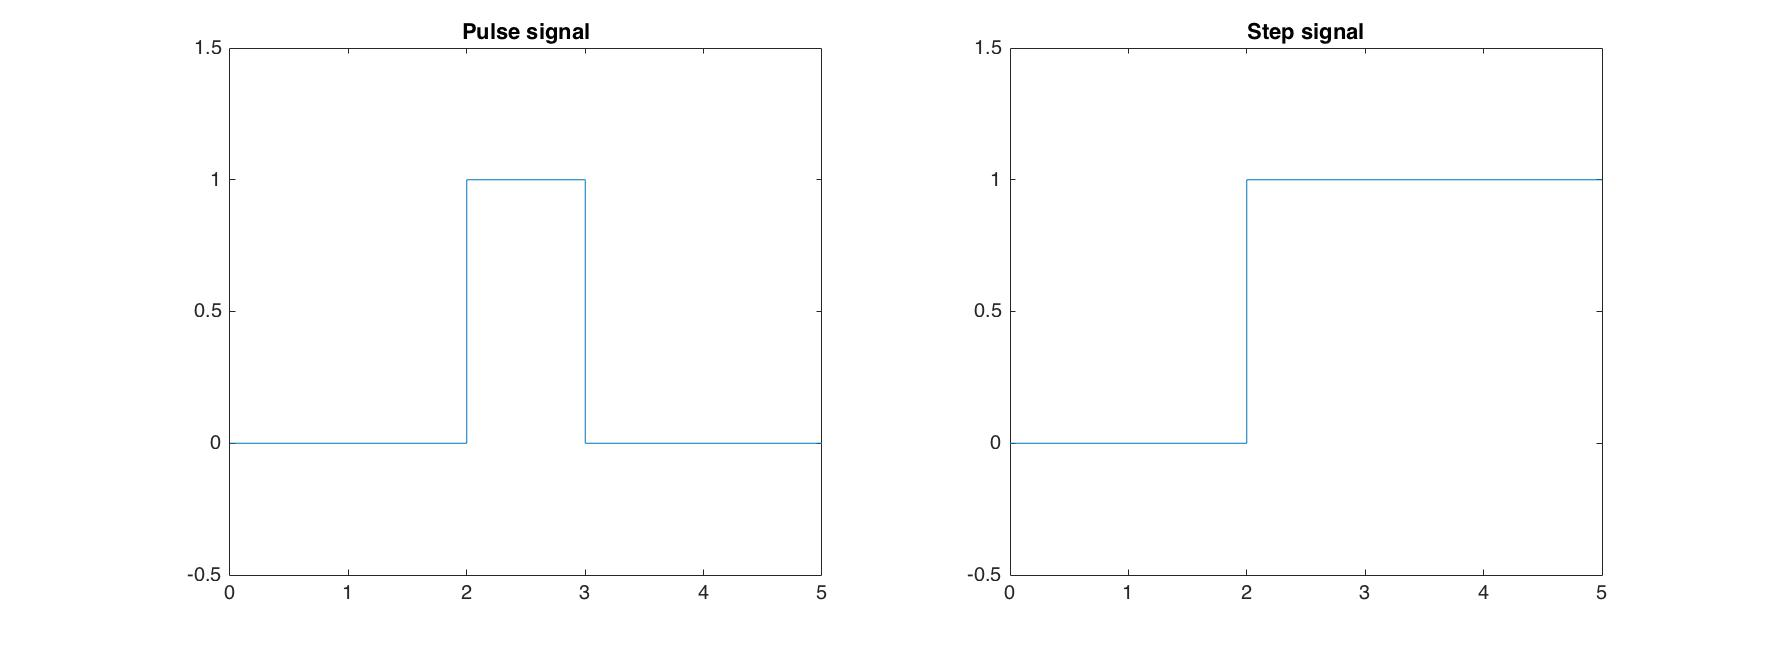
\includegraphics[width=7cm]{fig/step_pulse.jpg}
  %\fbox{\rule[-.5cm]{0cm}{4cm} \rule[-.5cm]{4cm}{0cm} }
  \caption{Pulse-like and step-like signal.}
  \label{fig1}
\end{figure}
% as $H(0)$
Now denote the \hba\  as $H(0)$ before $G$ increases and denote the \hba\ after $G$ increases as $H(n),\ n > 0$. The index corresponds to $G(n)$. For the step-like sequence $G$, the output \hba\ should increase with a slower and slower rate as time goes, since $(H(n)-H(n-1)) \propto F(\geq n\Delta t)$, which means that the increment difference between neighboring \hba\ measurements should be proportional to the fraction of the cells that do not have the same glycation rate in their whole life, i.e., those cells whose age is at least $n\Delta t$. Thus the increment difference should be linear for uniform distribution and exponential for finite exponential distribution.

If we use pulse-like sequence $G$, the output \hba\ should be expected to increase at the pulse and then decrease afterwards due to resetting the glucose concentration. Specifically, $H(n)\propto F(\geq n\Delta t)$, which means \hba\ is proportional to the fraction of cells that have been influenced by the impulse. The fraction is decreasing because cells are subject to death constantly. Thus $H(n)$ should decrease linearly for uniform distribution and exponentially for finite exponential distribution.

\subsection{Linear programming for generic distribution}
As soon as we represent the integral as Riemann sum, we can denote the problem by linear programming.
To simplify the notation, as in the above section, let $H(t)$ be $\hba(t)$ and $F(t)$ be $1-\tilde{F}_{\mathrm{RBC}_\mathrm{age}}(t;\theta)$ where $\tilde{F}_{\mathrm{RBC}_\mathrm{age}}(t;\theta)=\int_0^{t}\f(\tau)\dd \tau$ is the cumulative distribution function of the blood cell age distribution, which is controlled by the parameter $\theta$. At this moment, conforming to the previous assumptions, we assume that $\theta$ does not change over time and is an unknown constant.
%, which means the distribution does not change over time

Now suppose we can measure multiple $H$s and $G$s. The best case would be one measurement of $G$ and there is one corresponding measurement of $H$ at the same time.

The following equations is an approximation of equation \ref{h-conv}. 
\begin{align*}
\tilde{H}(0) = \frac{H(0)-1.627}{c\cdot \Delta t} & = G(0)F(0) + G(-1)F(1) + ... + G(-n)F(n) \\
\tilde{H}(1) = \frac{H(1)-1.627}{c\cdot \Delta t} & = G(1)F(0) + G(0)F(1) + ... + G(-(n-1))F(n) \\
\quad...\\
\tilde{H}(n) = \frac{H(n)-1.627}{c\cdot \Delta t} & = G(n)F(0) + G(n-1)F(1) + ... + G(0)F(n) 
\end{align*}
which is essentially a linear system and is equivalent to the matrix form,
\[\tilde{G}\cdot F = \tilde{H}\]
where $1=F(0)\geq F(1)\geq ...\geq F(n)\geq 0$ performs as the  constraint in order for $F$ to be a valid cumulative distribution function.

The only problem left is to specify the support size $n$ of the age distribution. So we can construct a linear programming (LP) with the objective function to minimize the distance between $F(n)$ and 0. But before reaching the final optimization problem, the constraints need to be represented in matrix form.

The constraint $1=F(0)\geq F(1)\geq ...\geq F(n)\geq 0$ can be rewritten as 
\begin{align*}
F(0) & = 1\\
F(0)-F(1) &\geq 0 \\
F(1)-F(2) &\geq 0 \\
\quad ... \\
F(n-1)-F(n) &\geq 0 \\
F(n) &\geq 0
\end{align*}
which is equivalent to the form $AF\geq 0$ and $F(0)=1$ where $A$ is a band matrix
\[A = 
\begin{bmatrix}
1 &-1 & 0 & ... & 0 \\
0& 1 & -1 & 0 & ... \\
...\\
0 & 0&... &0 & 1
\end{bmatrix}.
\]

The final constrained problem is
\begin{align*}
\min_{F}\ &(c\T F) \\
\st & \tilde{G}F = \tilde{H} \\
& AF \succeq 0\\
& F(0) = 1
\end{align*}
where $c = (0,...,0,1)\T\in\R^n$, $A\in\R^{n\times n}$, $\tilde{G}\in\R^{n\times n}$, $F\in\R^n$, and $H\in\R^n$.

Note that too many constraints may make the optimization problem infeasible. If that happens, we can reduce the constraints in $\tilde{G}$ to expand its null space. Another thing is that there might be different solutions for different support size $n$, so it is interesting in the future to determine under which condition the solution is unique for some $n$ and which distribution is optimal among different $n$'s.

\subsection{Pointwise deconvolution}
New signal comes in continuously at any time. So if we want to get the correct output sequence, we have to eliminate the previous signal effects, through which we may be able to do the pointwise deconvolution. But in practice, this is not possible, since what we can get are always part of the convolution results. For example, given $F = [1,0.8,0.6,0.4,0.2]$, we have a glucose sequence G as 
$G = [ 9  , 8 ,  7 ,  6 ,  5 ,  4 ,3 ,2 ,1]$ and the corresponding H measured at points when $G=5,4,3,2,1$ as $H = [19, 16, 13, 10, 7]$. However, the true convolution results of $F$ and $G$ are $\hat{H}=[9,   15.2,   18.8,   20,   19, 16,   13,   10,    7,    4,    2, 0.8,    0.2]$ where we only have part of the results in practice, so the pointwise deconvolution is not possible. Approximation techniques from Fourier analysis lie in the future work.


\section{Experiments}
In practice, we can only measure the glucose concentration $G$ up to some finite samples and sometimes the sample length cannot cover the support size of the density distribution. Thus in order to perform the simulations, we need to suppose the $G(t)$ is circulant, i.e., we extend the measurement sequence periodically. The simulation sequence is collected from the PhysioNet dataset by \citet{goldberger2000physiobank}. To simplify the process, we ignore the practical interval between measurements and take the interval as 1 day, in other words, we take $\Delta t = 1$.

Here is a sample used in the experiments. $G[n] = $ [135, 140, 169, 215, 224, 201, 265, 252, 332, 325, 296, 240, 285, 294, 276, 273, 296, 286, 349], where the last entry is the latest measurement. The \hba\ is computed as 10.5\% by equation \ref{ag-h} from the mean of glucose concentration $\E[G]\approx255.42$mg/dL.

\subsection{Uniform distribution}
The experiments in this section explore 1) the possibility of computing the parameter $\mean$ and 2) the importance of the bias term in equation \ref{h-conv}.

Notice that in equation \ref{r-uni}, it is hard to represent the parameter $\mean$ by \hba\ and $G(n)$ analytically. So as an alternative, we can enumerate $\mean$ and compute the corresponding $\hba_{\mean}$ and then select $\mean$ that gives the closed value to \hba, i.e., 
\[\hat{\mean} = {\arg\min}_{\mean}\left(\hba - \hba_{\mean}\right)^2.\]

We take 10 sequences of glucose concentration and compute the corresponding average glucose, \hba, $\mean$ with and without the bias term. The results are shown in Table \ref{sample-table}. From the table, it can be seen that $\mean$ with bias is much more consistent for patients both with diabetes or non-diabetes, and the standard deviation is $1.77$ days. On the other hand, for $\mean$ without bias term, the standard deviation is $6.34$ days.
It shows that there is not huge difference from person to person as to age distributions, so we can compute the overall density function under the assumption of uniform distribution,
\[\f(t) = \frac{1}{100.6},\quad\quad0\leq t\leq 100.6.\]

\begin{table}[t]
  \caption{Results of computed $\mean$ for uniform distribution}
  \label{sample-table1}
  \centering
  \begin{tabular}{ccccc}
    \toprule
    id     &   Average Glucose (mg/dL)   & \hba\ (\%)     & $\mean$ w/ bias (days) & $\mean$ w/o bias (days) \\
    \midrule
    1 & 255.42  & 10.5 & 49 & 58   \\
    2 & 174.29  &  7.7  & 51 & 65   \\
    3 & 133.56  &  6.3  & 49 & 67   \\
    4 & 128.86 & 6.1 & 48 & 65   \\
    5 & 105.86 & 5.3 & 51 & 74   \\
    6 & 108.24 & 5.4 & 50 & 72   \\
    7 & 108.05 & 5.4 & 53 & 75   \\
    8 & 110.40 & 5.5 & 52 & 74   \\
    9 & 120.05 & 5.8 & 52 & 73   \\
    10 & 225.11 & 9.5 & 48 & 59   \\
    \bottomrule
  \end{tabular}
\end{table}

\subsection{Distinguishing uniform distribution from finite exponential distribution}
The simulation takes an age distribution with support of 5 days. The setting is the same as in the previous simulation unless specified. Here the pdf of the uniform distribution is 
\[\f^{u}(x) = \frac{1}{5}, \quad x\in[0,5]\]
and the pdf of the finite exponential distribution is
\[\f^{e}(x) = \frac{e^{-x}}{1-e^{-5}}, \quad x\in[0,5]\]

The glucose concentration is increased from 100 mg/dL to 150 mg/dL and kept constant for step-like signal while decreased to 100 mg/dL after 1 day for pulse-like signal. The results are plotted in Figure \ref{fig2}. 

\begin{figure}[h]
  \centering
  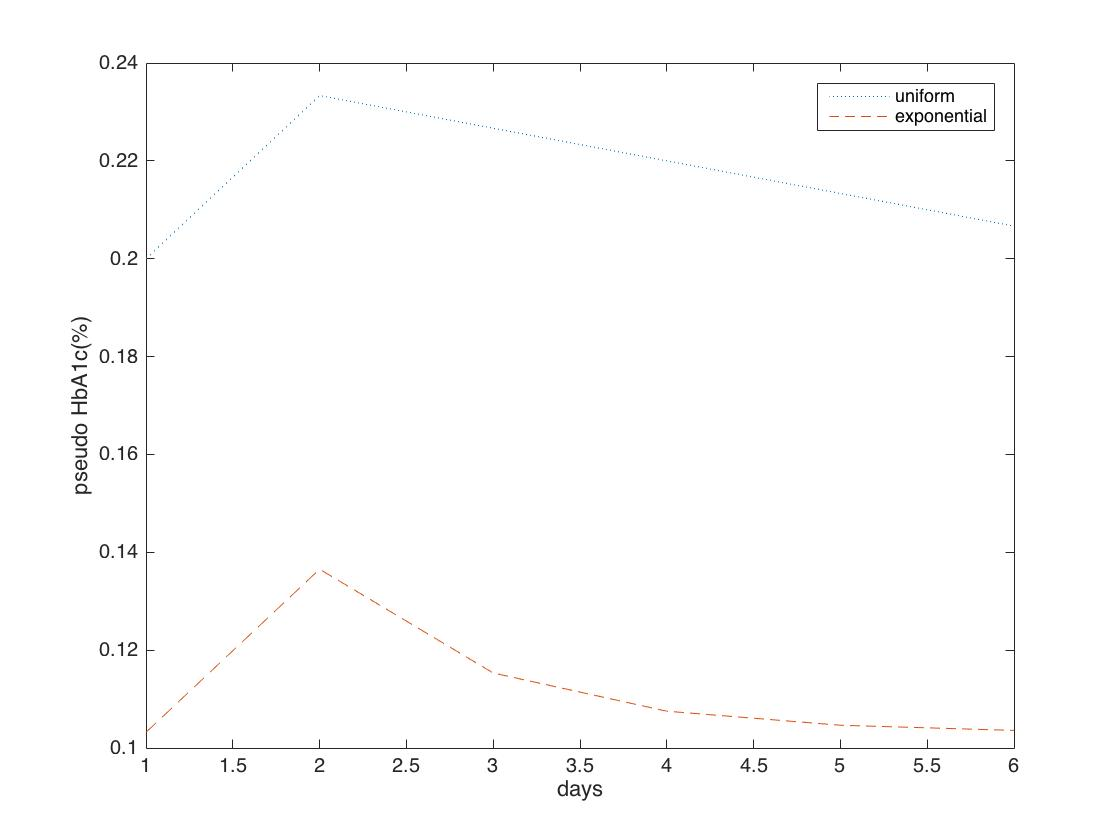
\includegraphics[width=5.5cm]{fig/distinguish_uni_exp_pulse.jpg}
  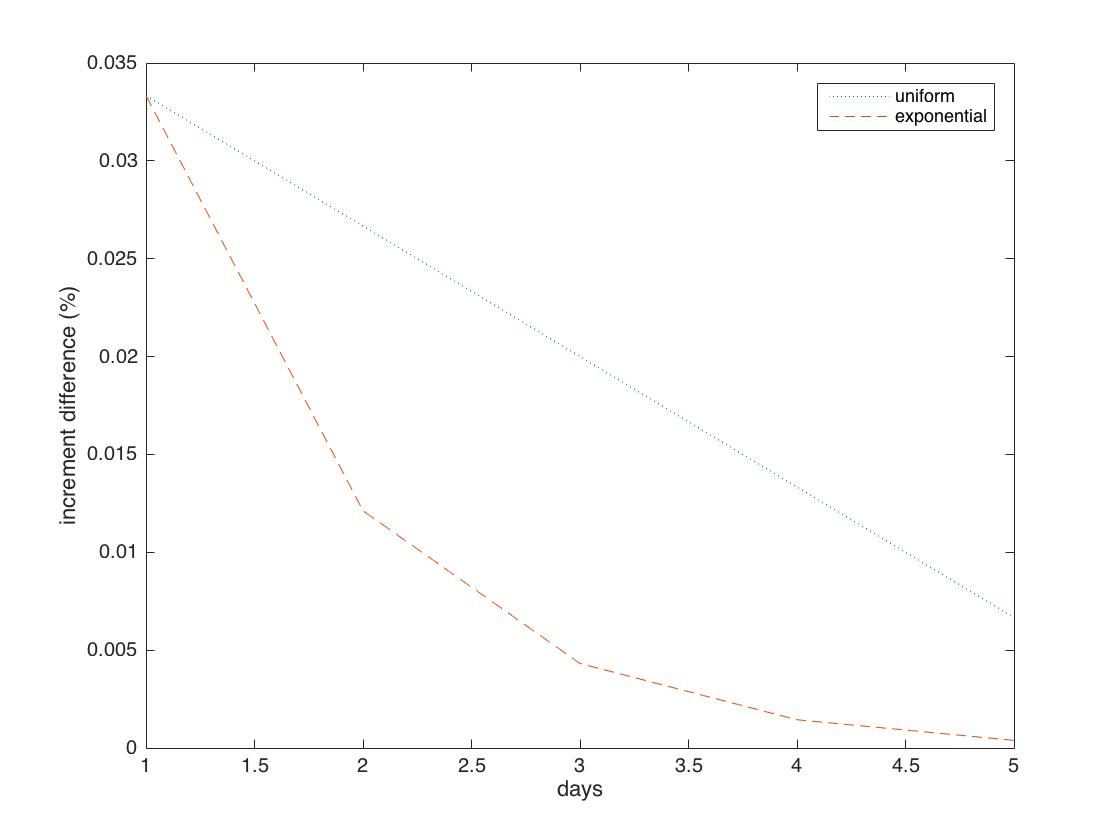
\includegraphics[width=5.5cm]{fig/distinguish_uni_exp.jpg}
  %\fbox{\rule[-.5cm]{0cm}{4cm} \rule[-.5cm]{4cm}{0cm} }
  \caption{The left figure is for pulse-like signal and the right figure is for step-like signal.}
  \label{fig2}
\end{figure}

For the pulse-like signal, the left one in Figure \ref{fig2} shows that the pseudo\footnote{The reason why we call it ``pesudo'' is that it equals to the true \hba\ up to a constant but that is enough to illustrate the effects.}  \hba\ increases at the pulse and then decreases linearly for uniform distribution and exponentially for finite exponential distribution. On the other hand, for the step-like signal, the day-by-day \hba\ increment difference is plotted in the right figure. It can be seen that the increment difference of the uniform distribution is decreasing linearly but the increment difference of the finite exponential distribution is decreasing exponentially.

Both these two kinds of signals can be attained easily in clinical environment and the experiment demonstrates that they can be used to distinguish distributions with different shapes.

\subsection{Linear programming optimization}
As in section 4.4, we construct the problem as equivalent to solving a constrained linear system, and we can solve it readily by current convex optimization softwares. For this experiment, we use  CVX from \citet{grant2008cvx}. We can try many different support size $n$ and plot them for comparisons.

In the experiments, if we specify too many constraints in matrix $\tilde{G}$, the problem my be infeasible. In an extreme case, we specify only one constraint in $\tilde{G}$ to see what happens.

It turns out that if we use the same sequence as in the previous section, we still get an infeasible problem. But if we set the sequence as randomly generated, it is feasible.
All the points are generated by the command \texttt{G=100+10*randn(2*n,1)}.


The cdf for $n=60,80,100,120,140$ is plotted in Figure \ref{fig3}. As $n$ increases, much density moves from old cells to young cells.  It is interesting to note that the approximatly uniform distribution when $n=100$ corresponds to our previous experiments in section 5.1, where we dictate a uniform distribution and also get $n\approx 100$.
\begin{figure}[h]
  \centering
  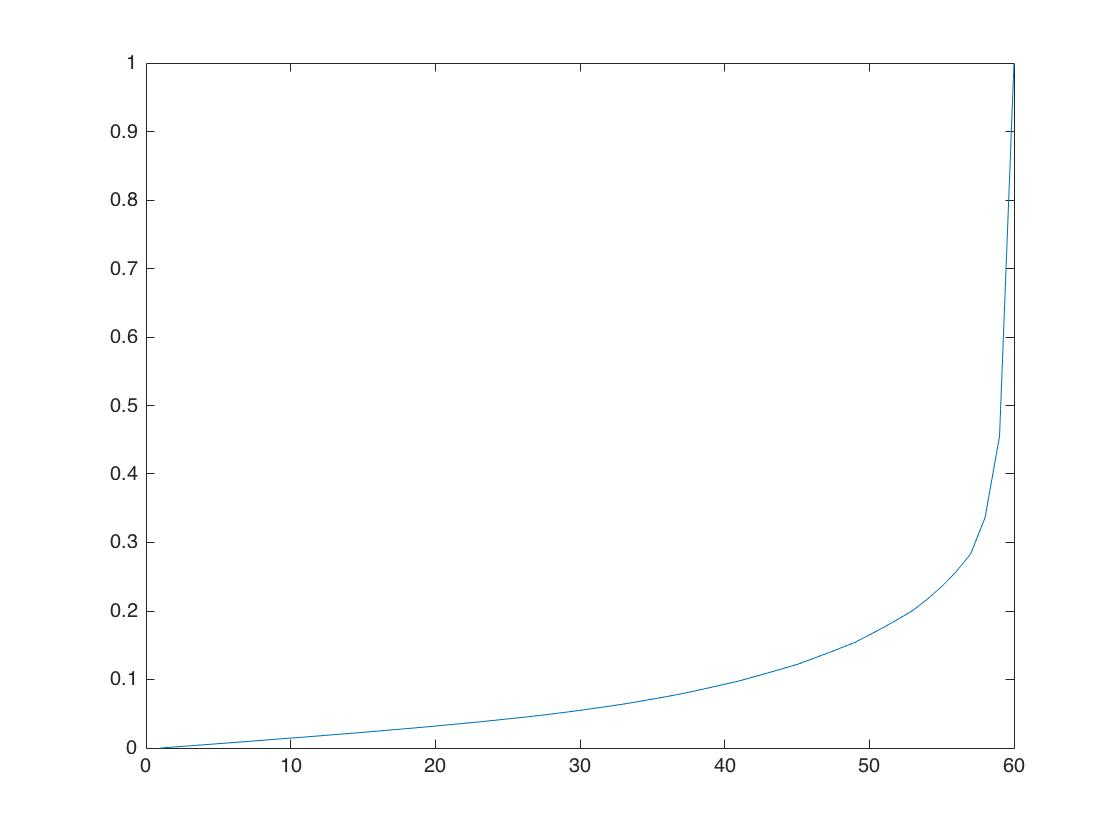
\includegraphics[width=2cm]{fig/60.jpg}
  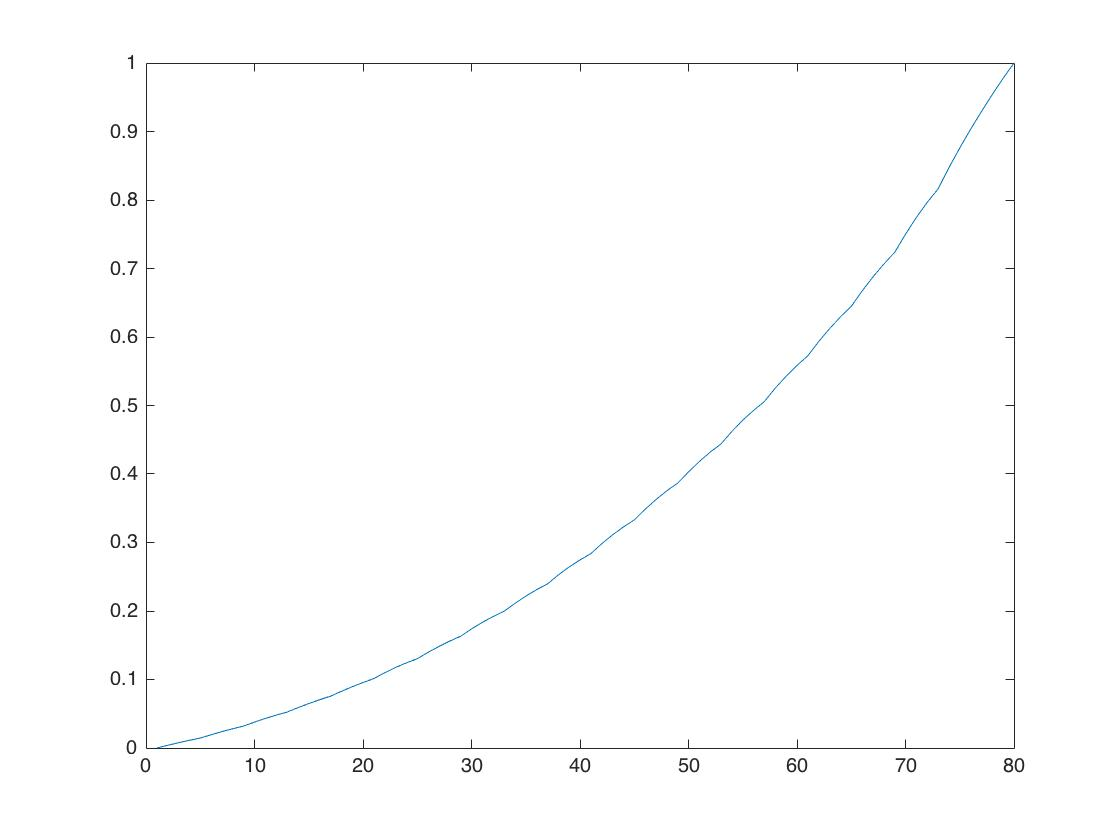
\includegraphics[width=2cm]{fig/80.jpg}
  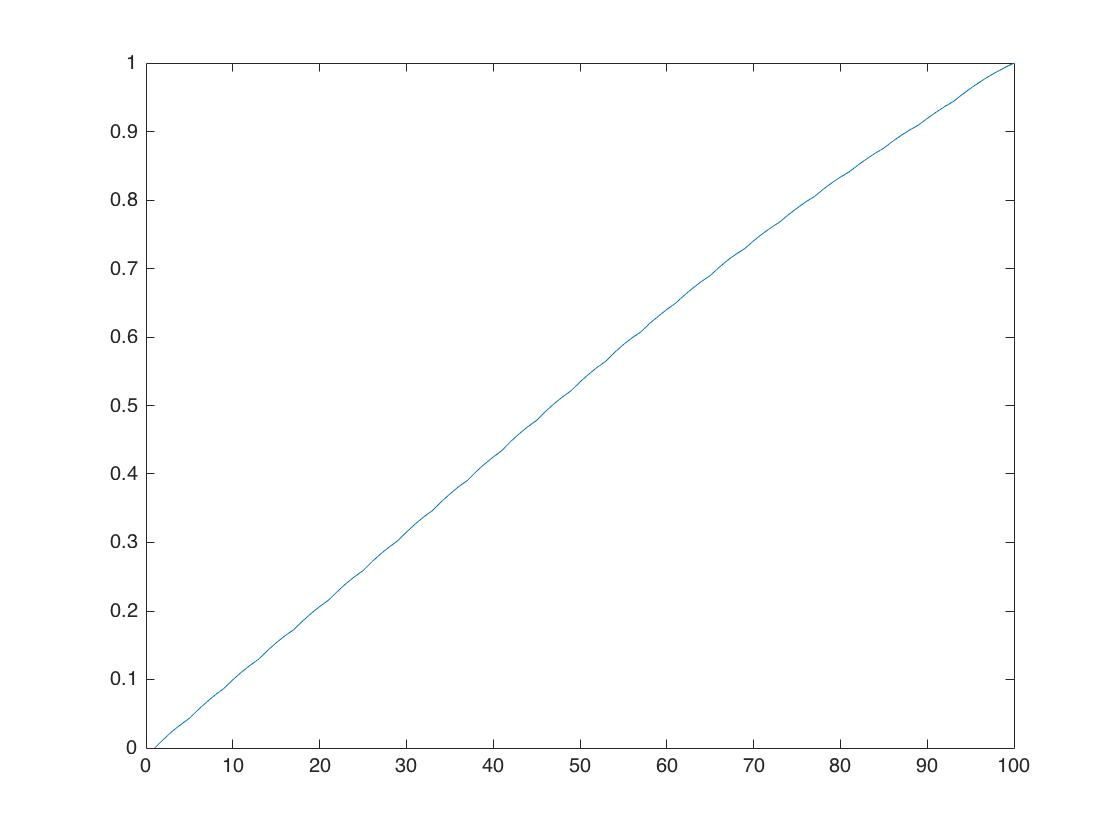
\includegraphics[width=2cm]{fig/100.jpg}
  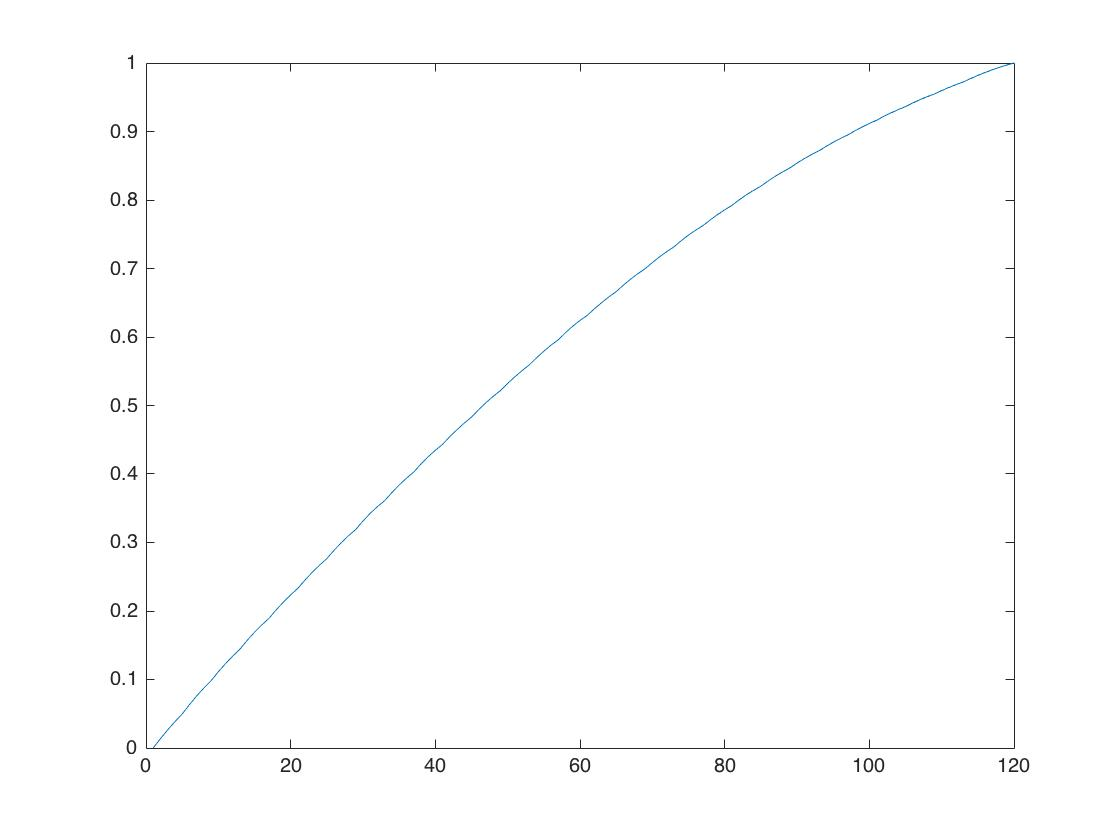
\includegraphics[width=2cm]{fig/120.jpg}
  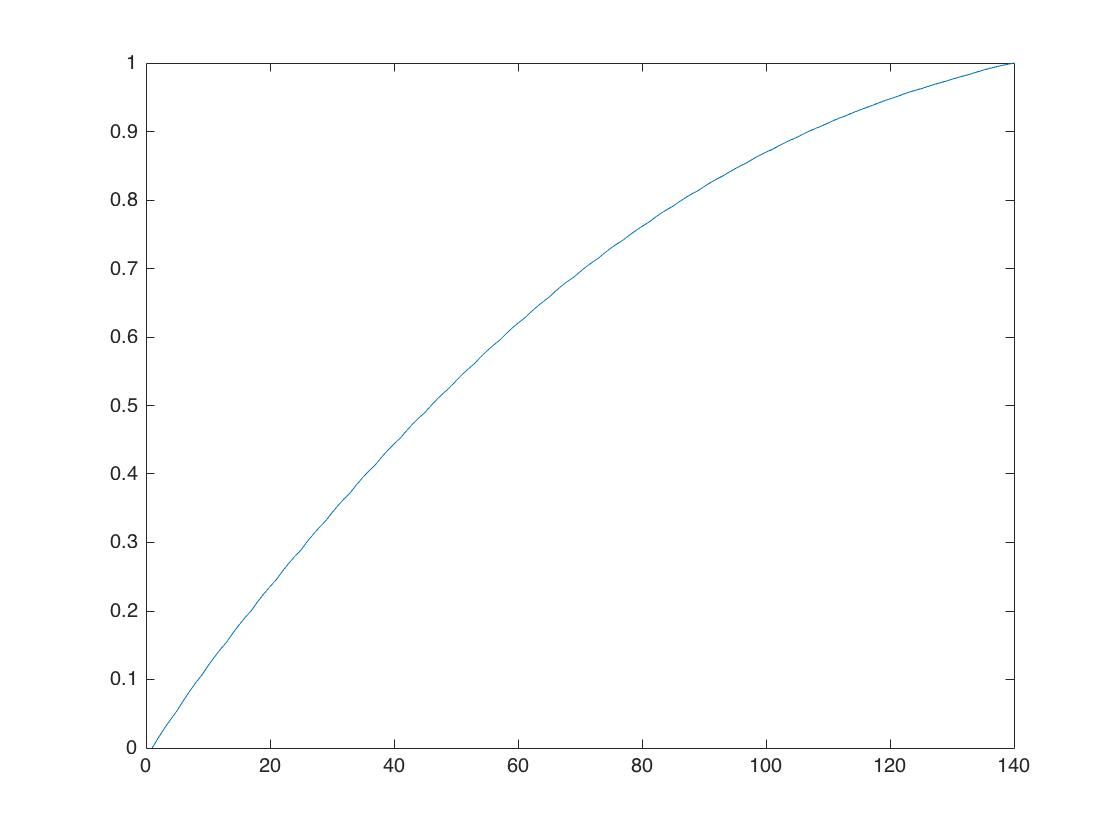
\includegraphics[width=2cm]{fig/140.jpg}
  %\fbox{\rule[-.5cm]{0cm}{4cm} \rule[-.5cm]{4cm}{0cm} }
  \caption{From left to right are the cdfs for $n=60,80,100,120,140$.}
  \label{fig3}
\end{figure}


\section{Future work}

1) It is obvious that the assumption of finite exponential distribution shall be investigated and experimented. 2) And the correction of the specification of the linear programming optimization problem should be further tested. It might be interesting to look into the conditions under which the solution is unique for some $n$ and which distribution is optimal among different $n$'s. 3) As pointed out in the previous section, the pointwise deconvolution is not possible even though we model the problem as a convolution equation. The approximation method in the frequency domain by using Fourier analysis is worth investigating.
%And deconvolution with Fourier analysis should be further analyzed. The current problems regarding the deconvolution may involve the incomplete outputs and the monotonic characteristic of the cdf of blood cells. Among them the incomplete-output problem stands out  because we do not have pointwise convolution outputs for two signals, not to say the pointwise deconvolution.

\section{Conclusion}
In this paper we define the connections between \hba, $G(t)$, and $\f(t)$ as a convolution operation. Necessary assumptions for feasible inference of $\f$ are provided. Experiments show that our proposed assumptions are consistent at least if the cell age distribution is uniform. Other theoretical aspects involving how to distinguish the uniform distribution and the finite exponential distribution, how to specify a linear programming problem for inferring a generic distribution, and the possibility of applying the pointwise deconvolution are also investigated.




%\subsubsection*{Acknowledgments}

%We would like to thank Chuyue Wu for helpful discussion about the backgrounds.



\bibliographystyle{plainnat}
\bibliography{ref.bib}


\end{document}
